\documentclass{article}
\usepackage{nameref,hyperref}
\newcommand{\beginsupplement}{%
	\setcounter{table}{0}
	\renewcommand{\thetable}{S3\arabic{table}}%
	\setcounter{figure}{0}
	\renewcommand{\thefigure}{S3\arabic{figure}}%
}
\beginsupplement


\usepackage{lastpage,fancyhdr,graphicx}
\newcommand{\ops}{\textsc{ops}}
\newcommand{\opsi}{O\textsc{ps}}
\newcommand{\vcps}{\textsc{vcps}}
\newcommand{\owl}{\textsc{owl}}
\newcommand{\owli}{O\textsc{wl}}
\newcommand{\sparql}{\textsc{s}par\textsc{ql}}
\newcommand{\bfo}{\textsc{bfo}}
\newcommand{\dbpedia}{\textsc{db}pedia}
\newcommand{\foaf}{\textsc{foaf}}
\newcommand{\ict}{\textsc{ict}}
\newcommand{\html}{\textsc{html}}
\newcommand{\node}{\textsc{n}ode.js}
\newcommand{\facebook}{\textsc{f}acebook}
\newcommand{\twitter}{\textsc{t}witter}
\newcommand{\wwwc}{\textsc{w3c}}
\newcommand{\skos}{\textsc{skos}}
\newcommand{\etherpad}{\textsc{e}therpad}
\newcommand{\ogp}{\textsc{ogp}}
\newcommand{\iri}{\textsc{iri}}
\newcommand{\uri}{\textsc{uri}}
\newcommand{\urii}{U\textsc{ri}}
\newcommand{\urll}{\textsc{url}}
\newcommand{\ngo}{\textsc{ngo}}
\newcommand{\http}{\textsc{http}}
\newcommand{\opa}{\textsc{op}a}
\newcommand{\ocd}{\textsc{ocd}}
\newcommand{\ontologiaa}{\textsc{o}ntologiaa}
\newcommand{\obs}{\textsc{obs}}
\newcommand{\pubby}{\textsc{p}ubby}
\newcommand{\rdf}{\textsc{rdf}}
\newcommand{\mysql}{\textsc{m}y\textsc{sql}}
\newcommand{\aan}{\textsc{aa}}
\newcommand{\cidadedemocratica}{\textsc{c}idade \textsc{d}emocr\'atica}
\newcommand{\participa}{\textsc{p}articipa.br}
\newcommand{\ontop}{\textsc{o}n\textsc{t}op}
\newcommand{\quest}{\textsc{q}uest}
\newcommand{\webprotege}{\textsc{w}ebprotege}
\newcommand{\obda}{\textsc{obda}}
\newcommand{\pnud}{\textsc{undp}}
\newcommand{\onu}{\textsc{un}}
\newcommand{\vbs}{\textsc{vbs}}
\newcommand{\lod}{\textsc{lod}}
\newcommand{\corais}{\textsc{c}orais}
\newcommand{\serpro}{\textsc{s}erpro}
\newcommand{\python}{\textsc{p}ython}
\newcommand{\protege}{\textsc{p}rot\`eg\`e}

\usepackage[margin=1em]{geometry}
\begin{document}
%\section{Glossary of terms, acronyms and abbreviations}\label{ap:glossary}
\vspace{-8cm}

Although deprecated, the figure bellow is the basis of \vcps\ and \ops. It is displayed here for completeness of exposition and as support for discussions within this article. 
\begin{figure*}[h]
    \centering
    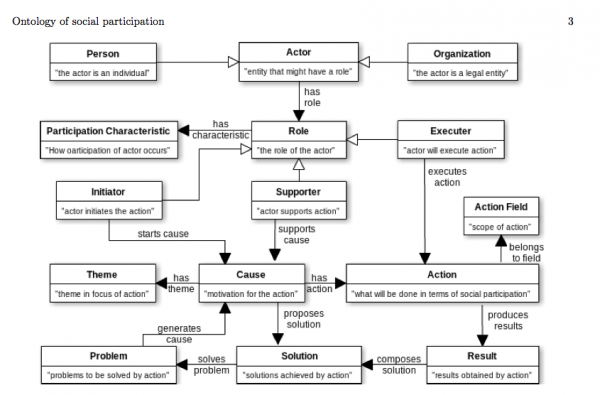
\includegraphics[width=0.8\textwidth]{../figs/diagramaOriginal}
    \caption{Original \vcps\ diagram. Although there were substantial \owl\ modifications, the main difference in the diagram is that the class \texttt{Role} was removed, as a \texttt{Role} is not able to start, execute or support anything. That is done by the Social Actor, as exposed in Figure~\ref{fig:v1}.}
    \label{fig:diaorig}
\end{figure*}


\end{document}
